\section{Supervised machine learning}
Machine learning er en underkategori af kunstig intelligens og en metode, der kan anvendes til at genkende mønstre i data. Da machine learning anvendes på en computer, er det muligt at bearbejde datasæt af en størrelse, der er uhåndterbare for mennesker at behandle. Det bruges mange steder og har mange formål, som f.eks. søgemaskiner, forudsigelse af aktiekurser og ansigtsgenkendelse.\cite{DIKU2010}


Et computerprogram er essentielt et sæt regler, udarbejdet manuelt af en programmør. Dette regelsæt afgør hvordan programmet opfører sig. Et almindeligt program som dette kan ikke afvige fra sit regelsæt og er derfor begrænset til programmørens evner.
Supervised machine learning tager derimod udgangspunkt i input-output relationer, hvorved modellen uafhængigt er i stand til selv at danne et regelsæt. En illustration af dette fremgår af \figref{ml}.


\begin{figure}[H]
%	\flushleft
	\centering
	\includegraphics[scale=0.8]{figures/machinelearning.png}
%	\flushleft
	\caption{\textit{Machine learning danner et regelsæt ud fra input-output relationen.\cite{DIKU2010}}}
	\label{ml}
	\end{figure}


En udvidelse af databasen, hvoraf regelsættet dannes fra, kan modellen blive mere nøjagtig. Dette gøres i en logisk proces, kaldet induktiv inferens, hvilket er en metode, hvor computeren tilnærmer sandsynligheden for et givent output, ud fra en sammenligning med lignende eksempler. Der findes forskellige måder at gøre dette på, men fælles for alle undersøges det, hvorvidt den nye data ligner den eksisterende data.\cite{DIKU2010}


\subsection{Supervised machine learning til estimering af indlæggelsesvarighed}
Ubalancen i kapacitetsudnyttelsen på ortopædkirurgisk afdeling på Aalborg Universitetshospital ønskes afhjulpet. Indlæggelsesvarigheden afhænger af mange forskellige faktorer, hvorfor det er uoverskueligt for en koordinator at planlægge samtlige patienters indlæggelsesvarighed. På nuværende tidspunkt anvendes ingen redskaber til estimering af dette, hvilket resulterer i ubalance i forholdet mellem aktivitet og kapacitet, der udgør kapacitetsudnyttelsen på afdelingen. 


Det anses muligt at planlægge patienter efter deres indlæggelsesvarighed for således at opnå en balance i kapacitetsudnyttelsen. Da koordinatorer ikke kan overkomme alle parametre for patienter kan det være fordelagtigt at anvende en prædiktiv model som et redskab til at estimere indlæggelsesvarigheden. Ved at anvende supervised machine learning til denne model, kan skjulte sammenhænge mellem parametre samt en stor datamængde håndteres\cite{DIKU2010}.

\subsection{Konstruering af model}
Machine learnings modeller konstrueres som en algoritme på baggrund af indsamlet data.\cite{Kuhn2013}  Når en algoritme designes til machine learning gøres dette på baggrund af et træningssæt. \cite{DIKU2010} 


\subsubsection{træningssæt}
Træningssættet tager udgangspunkt i en datamængde, der enten har kendte eller ukendte labels. Et træningssæt laves på baggrund af en del af den indsamlede data, hvor den resterende data testes på denne model. Et træningssæt basere på en forudbestemt machine learnings algoritme. Valget af algoritme belyses i afsnit \ref{algovalg}
Det er vigtigt at modellen ikke testes med samme data som anvendes til at opbygge træningssættet, da dette ville medføre at modellen kun er repræsentativ for den givne data.\cite{Kuhn2013} Ved supervised learning forsøges det at udarbejde en model, hvor data tilknyttes til labels og det bliver klassificeret. Det er vigtigt, at modellen afbildes så korrekt som muligt, for både træningssættet og de nye data. Et eksempel på udvælgelse af et træningssæts størrelse kunne være at udtage 200 datapunkter ud af 1000. Derefter konstrueres en algoritme på baggrund af træningssættet på 200 datapunkter, til at prædiktere en given parameter ud fra testsættet, hvilket er de resterende 800 datapunkter. Denne form for træningssæt opbygning er kendt som cross validation, og kan ses på figur \ref{fig:xval}\cite{Kuhn2013}.


\begin{figure}[H]
	%\flushleft 
	\centering
	\includegraphics[scale=.7]{figures/xval.png}
	%\flushleft
	\caption{\textit{Udvælgelse af datapunkter til træningssæt og testsæt.\cite{Kuhn2013}}
	\label{fig:xval}
\end{figure}


 Ved at variere hvilken del af datapunkterne der anvendes til træningssættet er der mulighed for at opnå en lavere fejl i træningssættet, og dermed en højere præcision af prædikteringen.\cite{Kuhn2013} 


\subsubsection{Algoritme valg} \label{algovalg}
I sammenhæng med at cross validere træningssættet med den resterende data, testes forskellige machine learnings algoritmer for at opnå den ønskede grad prædikterings præcision.\cite{Kuhn2013} Valget af algoritme baseres på størrelsen af fejlen mellem træningssæt og testsæt, og vurderes på samme grundlag som træningssættet. Variationen af machine learnings modeller betyder at nogle modeller er mere idéelle til bestemte datasæt end andre. Eksempelvis kan C4.5 modellen håndtere manglende data, således at imputering kan undgås. Når en algoritme med den ønskede præcision mellem trænings- og testsæt er fundet påbegyndes det sidste trin i konstruktionen af den prædiktive model, at finde et passende antal parametre bygge konstruere modellen ud fra.\cite{DIKU2010}    

\subsubsection{Bestemmelse af parametre}
Når en prædiktiv machine learnings model konstrueres, er det essentielt at have det korrekte antal parametre fra træningssættet. For få parametre betyder at sandsynligheden for fejl ift. prædikteringen af den ønskede output parameter er høj.Ved for mange parametre sker en over-fitting, hvor modellen bliver så specifik for træningssættet, således at testsættet prædikteres upræcist.\cite{DIKU2010} Fejlraten i en prædiktiv model, generaliseringsfejlen, kan ses på figur \ref{fig:genfejl}.


\begin{figure}[H]
%	\flushleft 
	\centering
	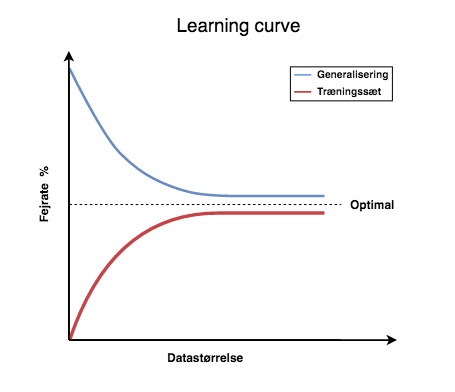
\includegraphics[scale=.5]{figures/genfejl.png}
	%\flushleft
	\caption{\textit{Learning curve der viser sammenhængen mellem datastørrelse og fejlrate.\cite{Kuhn2013}}
	\label{fig:genfejl}
\end{figure}

\noindent
Generaliseringsfejlen bygges også på hvor stort trænings og testsættet er. Generaliseringsfejlen er dog eksponentielt faldende, og kan dermed ikke undgås helt, uafhængigt af træningsættets størrelse.\cite{DIKU2010}
Antallet af parametre, og hvilke der har størst indflydelse på outputtet testes ved at opbygge træningssæt med et begrænset antal parametre, og derefter prædiktere ud fra testsættet. Ved at anvende alle mulige kombinationer af parametre, kan der konstrueres en model. Denne model anvender de parametre der i sammenhæng har størst indflydelse på outputtet, med det lavest mulige antal parametre. Dermed kan machine learning anvendes til at vurdere hvilke parametre der har en statistisk sammenhæng, og bør inddrages i en model til eksempelvis prædiktering af indlæggelsesvarighed.\cite{Kuhn2013,DIKU2010} 